\section{Experimental Evaluation}
\label{sec:parmaeval}

We evaluate the performance of PARMA using Amazon's Elastic
MapReduce platform. We used instances of type \emph{m1.xlarge}, which
contain roughly 17GB of memory and 6.5 EC2 compute units.
For data, we created artificial dataset using the synthetic data
generator from~\citep{ARTool}. This implementation is based on the
generator described in~\citep{AgrawalS94}, which can be parameterized to generate a wide
range of data. We used two distinct sets of parameters to generate the
datasets: the first set, shown in Table~\ref{tab:param1}, for the experiments
comparing PARMA and the distributed counting algorithm
(DistCount), and the second set, shown in Table~\ref{tab:param2},
for the experiments comparing PARMA and PFP.
The parameters were
chosen to mimic real-world datasets on which PARMA would be run. For a
full description of the relevant parameters, we refer the reader to
\citep{AgrawalS94}.  
The reason we needed two distinct datasets is that DistCount did not scale to
the larger dataset sizes,  as the amount of data it generates in the map phase
grows exponentially with the length of the individual transactions in the
dataset.  We found that DistCount would run out of memory using datasets with
longer transactions, and we had to generate datasets with both shorter and less
transactions for its comparisons. 
%This is a strong
%testament to the lack of scalability of the distributed counting
%algorithm.  

Because PARMA is an approximate algorithm, the choice of accuracy
parameters $\varepsilon$ and $\delta$ are important, as is $\theta$,
the minimum frequency at which itemsets were mined. In all of our
experiments, $\varepsilon = 0.05$ and $\delta = 0.01$. This means that
the collection of itemsets mined by PARMA will be an absolute 0.05-close
approximation with probability 0.99. In practice, we show later that the results
are much more accurate than what this. For all experiments other than the
minimum frequency performance comparison in Figure \ref{fig:parmafrequency} and for
the accuracy comparison in Figures~\ref{fig:parmaabsfreqerr}
and~\ref{fig:parmaconfintwidth}, $\theta$ was kept constant at 0.1.

\begin{comment}
We focus on three main aspects in the experimental analysis of PARMA. First is the runtime
analysis. In this set of experiments we compare PARMA to PFP and DistCount using several
different datasets of varying size and mined with varying minimum frequency thresholds. We
then break down the runtime of PARMA into the map, reduce and shuffle phases of each of
the two stages. This demonstrates which parts of the algorithm have runtimes that increase
as the data size grows and which parts are relatively data independent. The second aspect
is speedup, to show the scalability of our algorithm. In these experiments, data and
cluster size are varied to determine how PARMA scales. Finally, because the output of
PARMA is an absolute $\varepsilon$-close approximation of the real set of frequent itemsets, we provide
an accuracy analysis to verify that our results are indeed within the desired quality
bounds.
\end{comment}

\begin{table}[tb] \centering
\begin{tabular}{ l  r } \hline number of items & 1000 \\ 
average transaction length & 5 \\ 
average size of maximal potentially large itemsets & 5 \\ 
number of maximal potentially large itemsets & 5 \\
correlation among maximal potentially large itemsets & 0.1 \\
corruption of maximal potentially large itemsets & 0.1 \\ \hline
\end{tabular}
  \caption{Parameters used to generate the datasets for the runtime comparison between 
  DistCount and PARMA in Figure \ref{fig:parmaperformance}.}
  \label{tab:param1}
\end{table}

\begin{table}[tb] \centering
\begin{tabular}{ l  r } 
\hline 
number of items & 10000 \\ 
average transaction length & 10 \\ 
average size of maximal potentially large itemsets & 5 \\ 
number of maximal potentially large itemsets & 20 \\
correlation among maximal potentially large itemsets & 0.1 \\
corruption of maximal potentially large itemsets & 0.1 \\ 
\hline
\end{tabular}
  \caption{Parameters used to generate the datasets for the runtime comparison
  between PFP and PARMA in Figure \ref{fig:parmaperformance}.}
  \label{tab:param2}
\end{table}
Due to space limitations, we do not report the results of the experiments to
evaluate the performances of PARMA as the parameters of the optimization problem change.

\subsection{Performance Analysis} 

For the performance analysis of PARMA, we analyze the relative
performance against two exact FIM algorithms on MapReduce,
\emph{DistCount} and \emph{PFP}, on a cluster of 8 nodes. We also provide a breakdown of the costs
associated with each stage of PARMA.


Figure~\ref{fig:parmaperformance} (top) shows the comparison
between PARMA and DistCount.
\begin{comment}
As discussed previously, due to
limitations in the scalability of DistCount, we were unable to test on
the larger datasets, so the smaller datasets were generated using
parameters from Table \ref{table:param1}. 
\end{comment}
For DistCount,
longer itemsets affect runtime the most, as
the number of key/value pairs generated from each transaction is
exponential in the size of the transaction. This is not to say that more
transactions does not affect runtime, just that the length of those
transactions also has a significant impact. Because of this, it is
possible to have datasets with fewer transactions but with more ``long''
transactions that take longer to mine. This effect is seen in the first
three datasets (1-3 million). 
\begin{comment} 
Even though the number of transactions
significantly increases, the relative length of the longest transactions
was actually longer in the 1 million transaction dataset. Indeed, upon
further inspection, we found that the 1 million transaction dataset had
25 transactions over 20 items in length, while the 2 and 3 million
transaction dataset had less than 15. 
\end{comment}
Of course, since these datasets
were generated independently and with the same parameters,
this was purely by chance. However, as the number of transactions continues to
increase, the exponential growth in the number of intermediate key/value
pairs is seen by the sharp increase in runtime. While we tried to test
with a dataset with 6 million transaction, DistCount ran out of memory.
The lack of ability to handle either long individual transactions or a
large number of transactions in a dataset limits DistCount's
real-world applicability. 
\begin{comment}
The runtime of PARMA is significantly faster
than that of DistCount and, more importantly, nearly constant across
dataset sizes. The reasons for this will be discussed in detail later.
\end{comment}

\begin{figure}[htb]
  \centering
    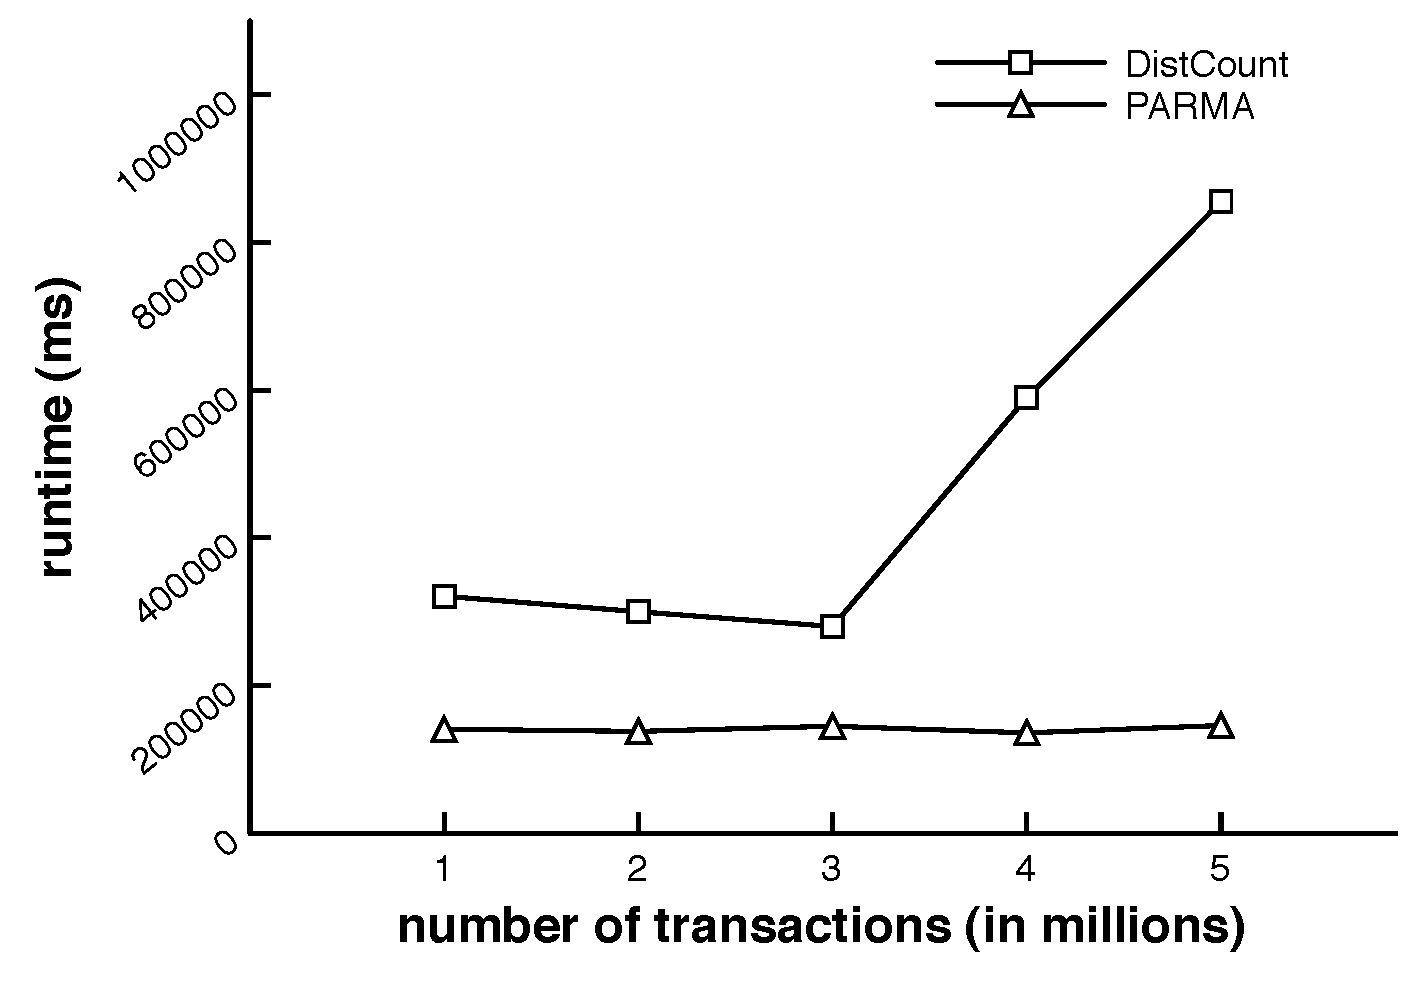
\includegraphics[width=0.49\textwidth]{parma/distributed_counting}
    \hfill
    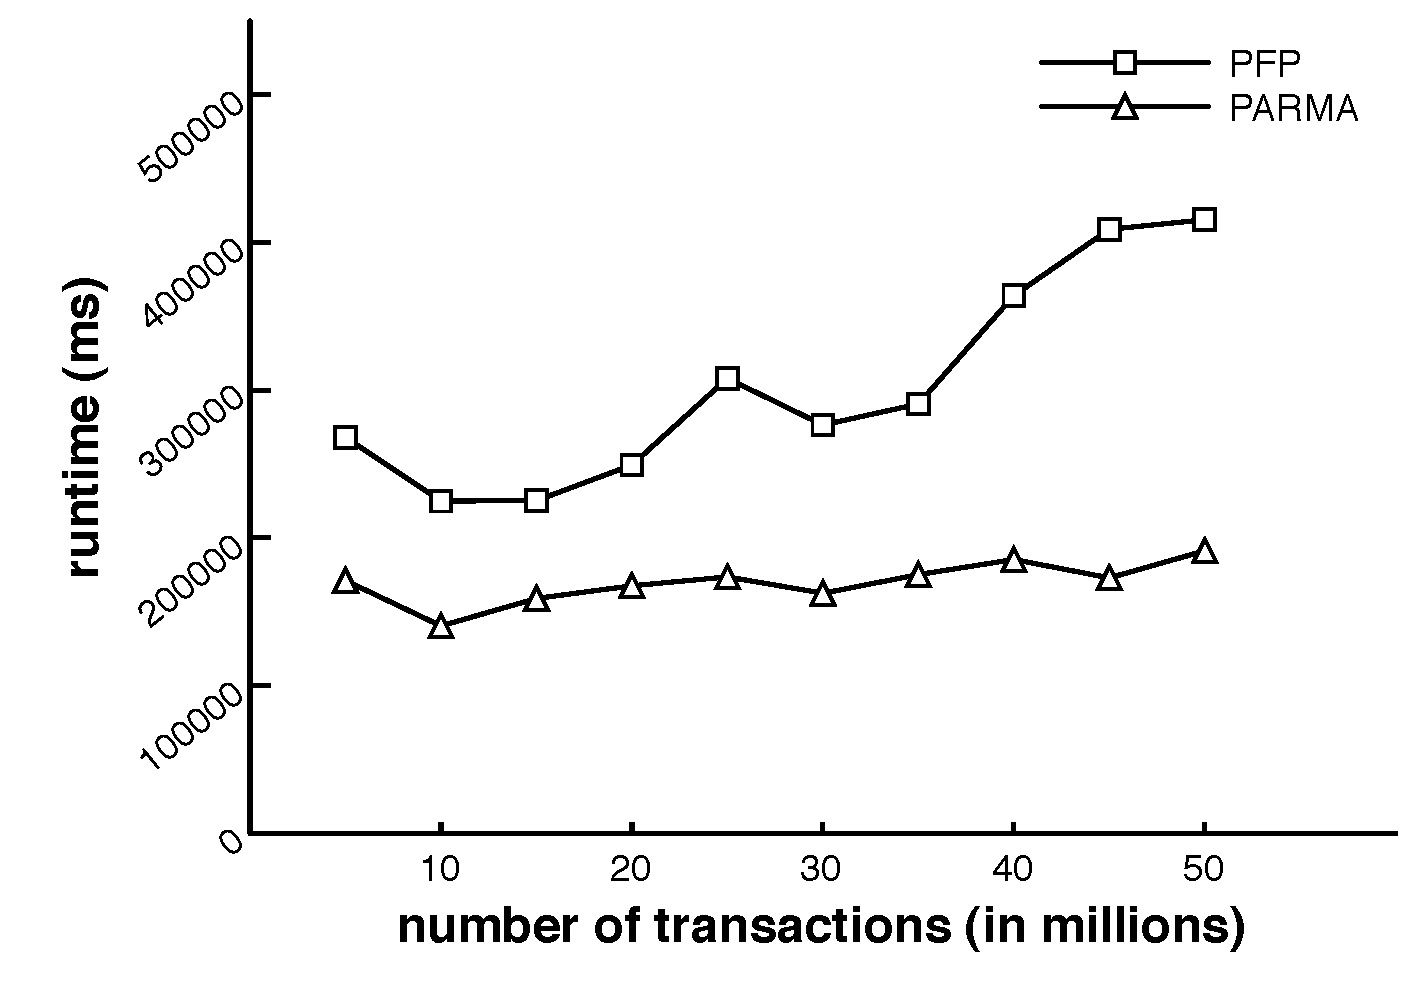
\includegraphics[width=0.49\textwidth]{parma/performance}
  \caption{A runtime comparison of PARMA with DistCount and PFP.}
\label{fig:parmaperformance}
\end{figure}

For the performance comparison with PFP, 10 datasets were generated
using parameter values from Table \ref{tab:param2} and ranging in size
from 10 to 50 million transactions.
The results are shown in
Figure~\ref{fig:parmaperformance} (bottom).
  For every dataset tested, PARMA was able
to mine the dataset roughly 30-55\% faster than PFP. The reason for the
relative performance advantage of PARMA is twofold. The first (and
primary) reason is that for larger datasets the size of the dataset that
PARMA has sampled (and mined) is staying the same, whereas PFP is mining
more and more transactions as the dataset grows. The second reason is
that as the dataset grows, PFP is potentially duplicating more and more
transactions as it assigns transactions to groups. A transaction that
belongs to multiple groups is sent to multiple reducers, resulting in
higher network costs.

The most important aspect of the comparison of PFP to PARMA is that the
runtimes as data grows are clearly diverging due to the reasons
discussed above. While 50 million transactions is very sizable, it is
not hard to imagine real-world datasets with transactions on the order
of billions. Indeed, many point-of-sale datasets would easily break this
boundary. In these scenarios a randomized algorithm such as PARMA would
show increasing performance advantages over exact algorithms such as any
of the standard non-parallel algorithms or PFP, which must mine the
entire dataset. At that scale, even transmitting that data over the
network (several times in the case of PFP) would become prohibitive.

To understand the performance of PARMA it is important to analyze the
runtimes at each of the various stages in the algorithm. To do this, we
have implemented runtime timers at very fine granularities throughout
our algorithm. The timers' values are written to Hadoop job logs for
analysis. This breakdown allows us to not only analyze the overall
runtime, but also the sections of the algorithm whose runtimes are
affected by an increase in data size. In Figure \ref{fig:parmabreakdown1}, a
breakdown of PARMA runtimes is shown for each of the six segments of the
algorithm, which include a map, shuffle and reduce phase for each of the
two stages. 
Due to space limitations, we only show the breakdown for a subset of
the datasets we tested. We observed the same patterns for all datasets.
This breakdown demonstrates several interesting aspects of
PARMA. First, the cost of the mining local frequent itemsets (stage 1,
reduce) is relatively constant. For many frequent itemset mining
implementations, this cost will grow with the size of the input. This is
not the case in PARMA, because local frequent itemset mining is being
done on constant-sized sample of the input. Indeed another interesting
observation, as expected, is that the only cost that increases as sample
size increases is the cost of sampling (stage 1, map). This is because
in order to be sampled the input data must be read, so larger input data
means larger read times. In practice, this cost is minimal and
grows linearly with the input, hence it will never be prohibitive,
especially considering all other current algorithms must read the entire
input data at least once, and in many cases multiple times. 

There is one outlier in the graph, which is the dataset with 5 million
transactions. Because each dataset was independently generated, it is
possible for a dataset to have a larger number of frequent itemsets than
other datasets, even if it has less transactions. This is the case with
the 5 million transaction dataset, which takes longer to run mine for both PARMA and PFP
due to the relatively greater number of frequent itemsets. 

\begin{comment}
To see that this is indeed what is
happening, we refer again to Figure \ref{fig:parmabreakdown1}. As expected,
the sample generation phase (stage 1, map) is smaller relative to the
larger datasets. However, the local frequent itemset mining phase (stage
1, reduce) is longer than any of the larger datasets. This is because
there are more frequent itemsets in that dataset. This can also be seen
in the relatively larger shuffle phase of stage 2, which is in charge of
sending all equivalent local frequent itemsets to the same reducer for
aggregation. Because there are more local itemsets present, this shuffle
stage is larger than for the other datasets. Because the same dataset
was used for the runtime of analysis of PFP and PARMA, and the overall
runtimes of both should increase in a dataset with more frequent
itemsets, we should see a higher runtime on the 5 million transaction
dataset for PFP relative to its the other datasets, which is indeed the
case. The runtime of PFP increases with both the size of the dataset as
well as the number of frequent itemsets present, but it is not until a
dataset of 25 million transactions that the runtime exceeds the runtime
for the 5 million transaction dataset. This outlier is not a flaw with
PARMA or PFP, but is a result of one of the inherent aspects of frequent
itemset mining: it takes longer to mine datasets with more frequent
itemsets.
\end{comment}

\begin{figure}[htb]
\centering
    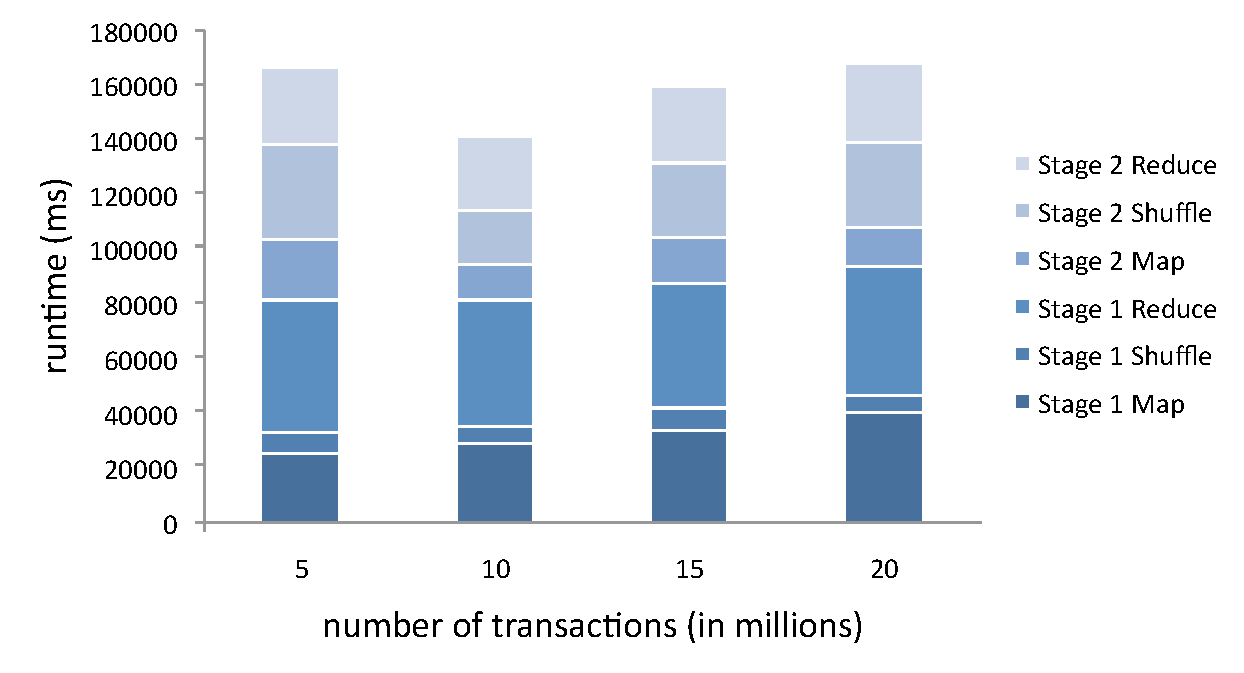
\includegraphics[width=0.75\textwidth]{parma/breakdown1}
  \caption{A comparison of runtimes of the map/reduce/shuffle phases
of PARMA, as a function of number of transactions. Run on
an 8 node Elastic MapReduce cluster.}
\label{fig:parmabreakdown1}
\end{figure}

\begin{figure}[htb]
  \centering
    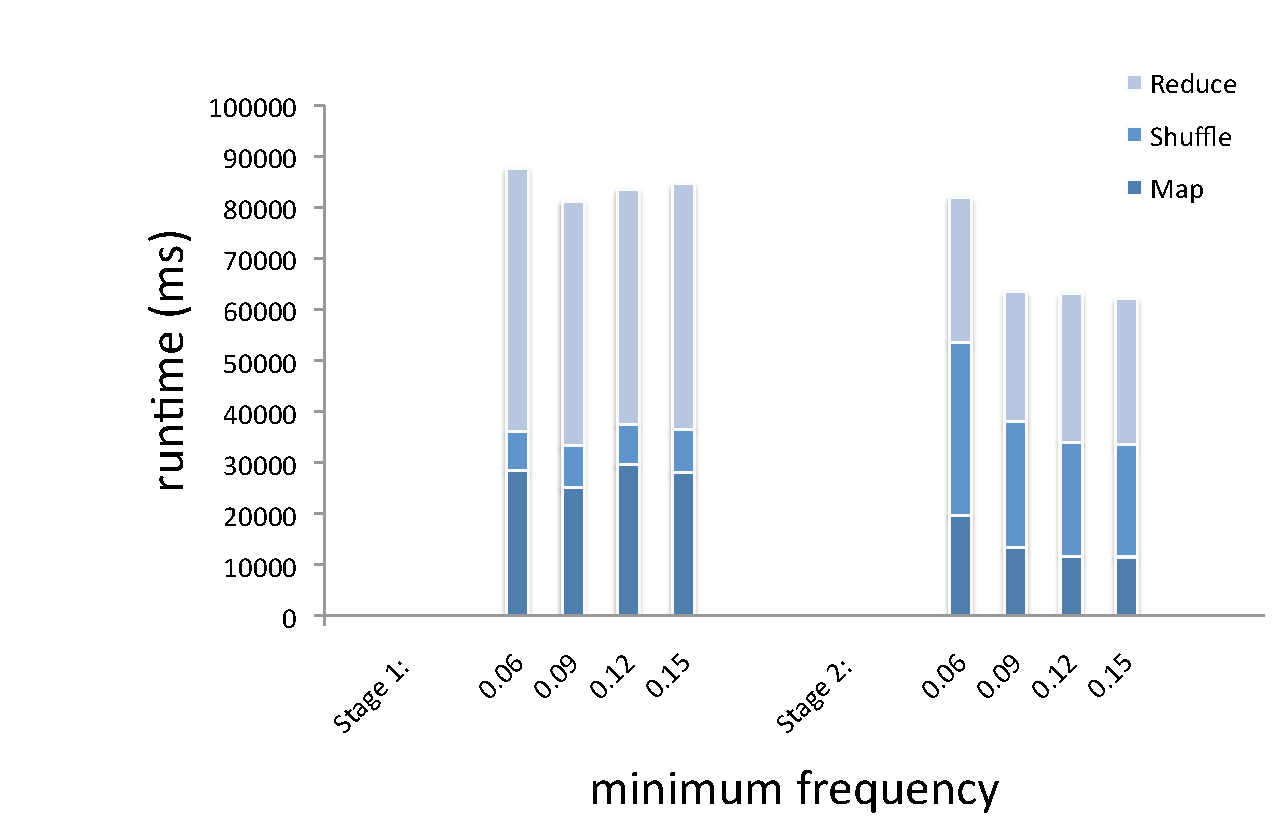
\includegraphics[width=0.75\textwidth]{parma/frequency}
  \caption{A comparison of runtimes of the map/reduce/shuffle phases
of PARMA, as a function of minimum frequency. Clustered by stage. Run
on an 8 node Elastic MapReduce cluster.}
\label{fig:parmafrequency}
\end{figure}


\begin{comment}
In Figure \ref{fig:parmabreakdown2}, a breakdown of total runtimes is shown
clustered by stage. In this view, it is apparent that most of the
phases of the algorithm are nearly constant across data sizes. The
obvious increase is the map of stage 1, which was discussed
above. Another slight runtime increase as data increases occurs in the
shuffle phase of stage 2. Because there are more transactions in the
larger datasets, there will be more frequent itemsets on average. In
stage 2, an identity mapper sends each frequent itemset to the
appropriate reducer for counting. Thus, all this data is being moved
across the network, which is manifested in the shuffle phase of stage
2. The more frequent itemsets, the more data there is to shuffle
across the network, which results in longer runtimes. Also, in
Figure~\ref{fig:parmabreakdown2} we once again notice that the 5 million
transaction dataset is an outlier. The longer than expected phase is
the shuffle phase of stage 2, which again suggests that this dataset
took longer to mine because more frequent itemsets were found.
\end{comment}

Figure \ref{fig:parmafrequency} shows the breakdown of PARMA runtimes as
the minimum frequency at which the data is mined at is changed. Data
size was kept constant at 10 million transactions. Minimum frequency
is used by the local frequent itemset mining algorithm to prune
itemsets; itemsets below the minimum frequency are not considered
frequent, nor is any superset since a superset must, by definition,
contain the not frequent set and therefore cannot be frequent
itself. Intuitively, a lower minimum frequency will mean more frequent
itemsets are produced. Other than a runtime increase in the local
frequent itemset mining phase (stage 1, reduce), the effects of this
can be seen in the stage 2 shuffle phase as well, as there is more
data to move across the network. Still, the added costs of mining with
lower frequencies are relatively small.

%\begin{figure}[htb]
 % \centering
 %   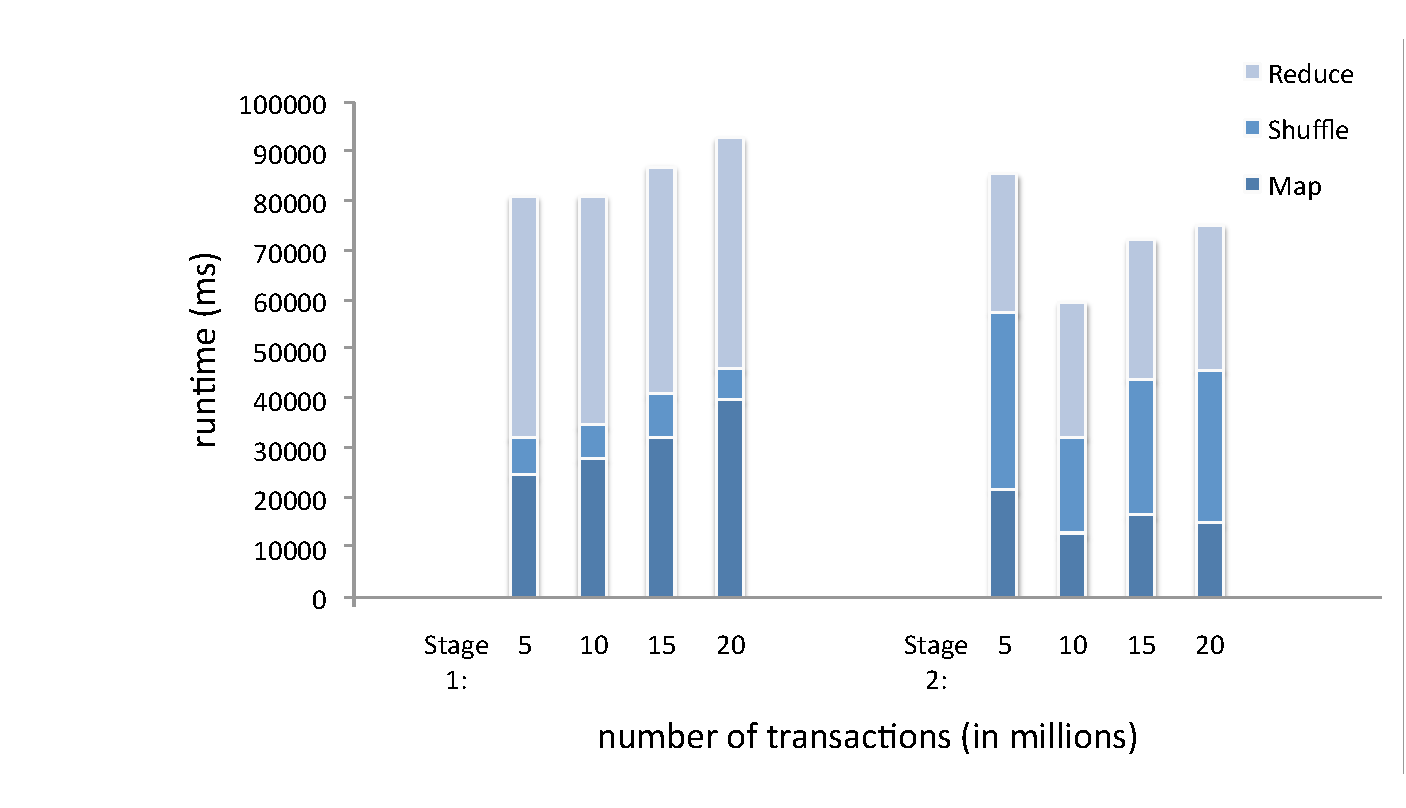
\includegraphics[width=0.4\textwidth]{breakdown2}
%  \caption{A Comparison of runtimes of the map/reduce/shuffle phases
%of PARMA, as a function of input dataset size. Clustered by stage. Run
%on an 8 node Elastic MapReduce cluster.}
%\label{fig:parmabreakdown2}
%\end{figure}

%\vspace{-10pt}
\subsection{Speedup and Scalability}
To show the speedup of PARMA, we used a two-nodes cluster as the
baseline. Because PARMA is intended to be a parallel algorithm, the choice of a
two-nodes cluster was more appropriate than the standard single node
baseline. For the dataset, we used a 10 million transaction database
generated using the parameters in Table \ref{tab:param2}. The results
are shown in Figure \ref{fig:parmaspeedup}. The three lines on this graph
represent the relative speedup of both stage 1 and stage 2 as well as
the overall PARMA algorithm. The graph indicates that stage 1 is highly
parallelizable and follows a near-ideal speedup for up to 8 nodes,
after which a slight degradation of speedup occurs. There are two
reasons for this slight degradation. In the map phase of stage 1, due
to an implementation decision in Hadoop, the smallest unit of data
that can be split is one HDFS block. As we continue to add more nodes
to the cluster, we may have more available map slots than HDFS data
blocks, resulting in some slots being unused. Theoretically, this
could be fixed by allowing smaller granularity splitting in
Hadoop. Another cause of the slightly sub-ideal speedup in stage 1 is
from the reducer. Because the data in this experiment was held
constant, the slight degradation in speedup as more than 8 nodes were
added was a result of an inefficient over-splitting of transaction
data. If each reducer in stage 1 is mining a very small subset of the
transactions, the overhead of building the FP-tree begins to dominate
the cost of mining the FP-tree. This is because the cost of mining the
FP-tree is relatively fixed. Thus, we can ``over-split'' the data by
forcing the reducer to build a large FP-tree only to mine a small set
of transactions. For larger samples, the size of the cluster where
speedup degradation begins to occur would also increase, meaning PARMA
would continue to scale.

\begin{figure}[thb]
  \centering
  \begin{subfigure}[b]{0.49\textwidth}
    \centering
    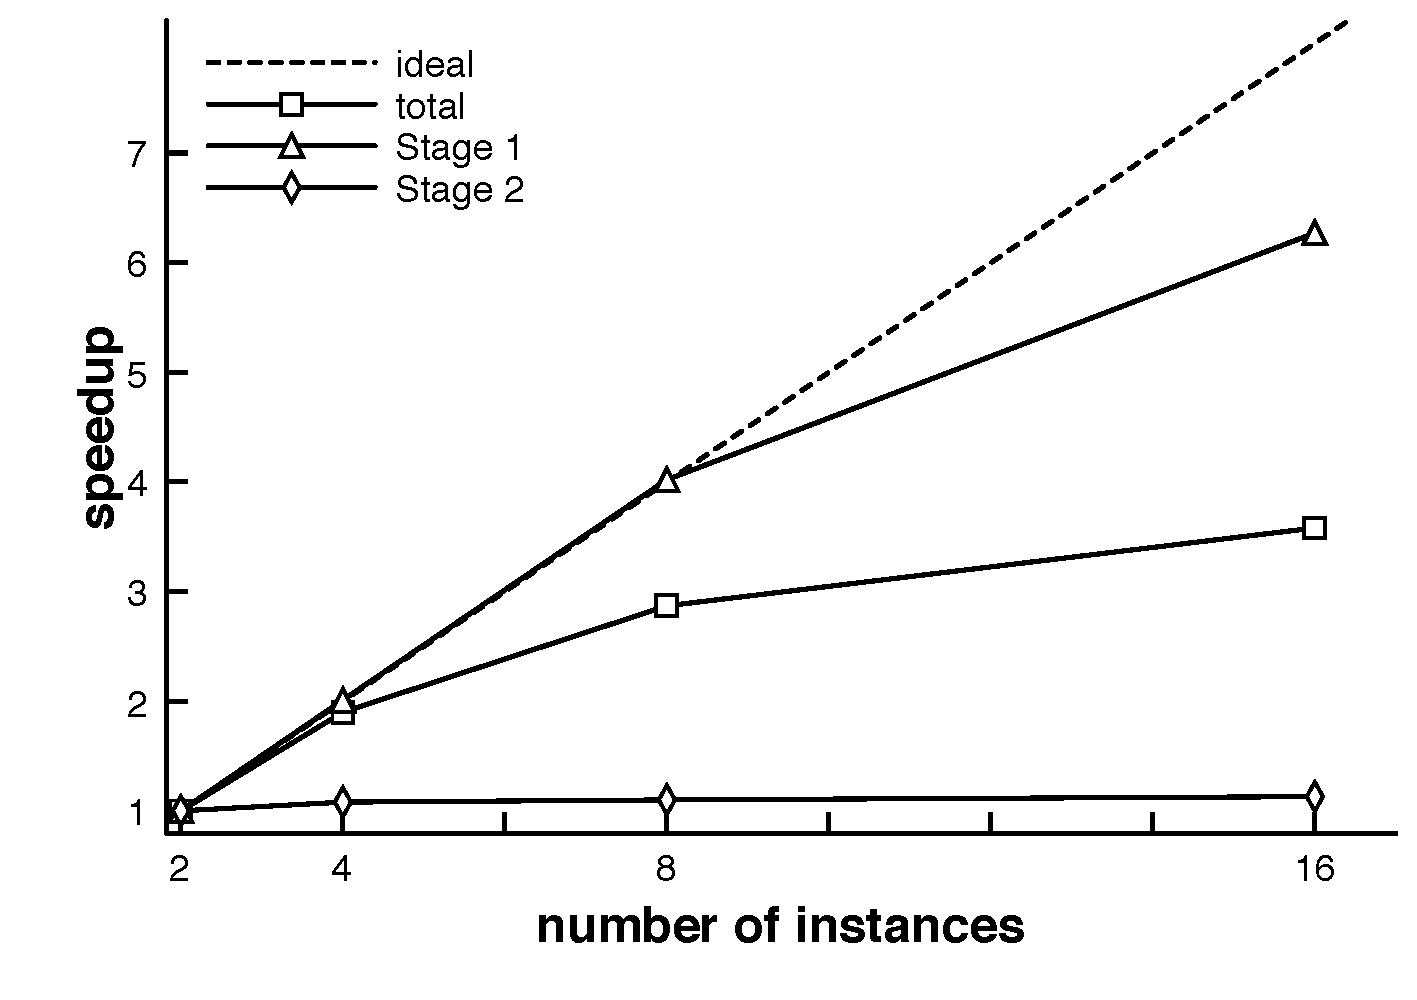
\includegraphics[width=\textwidth]{parma/speedup}
    \caption{Speedup analysis broken down by stages.}
    \label{fig:parmaspeedup}
  \end{subfigure}
  \hfill
  \begin{subfigure}[b]{0.49\textwidth}
    \centering
    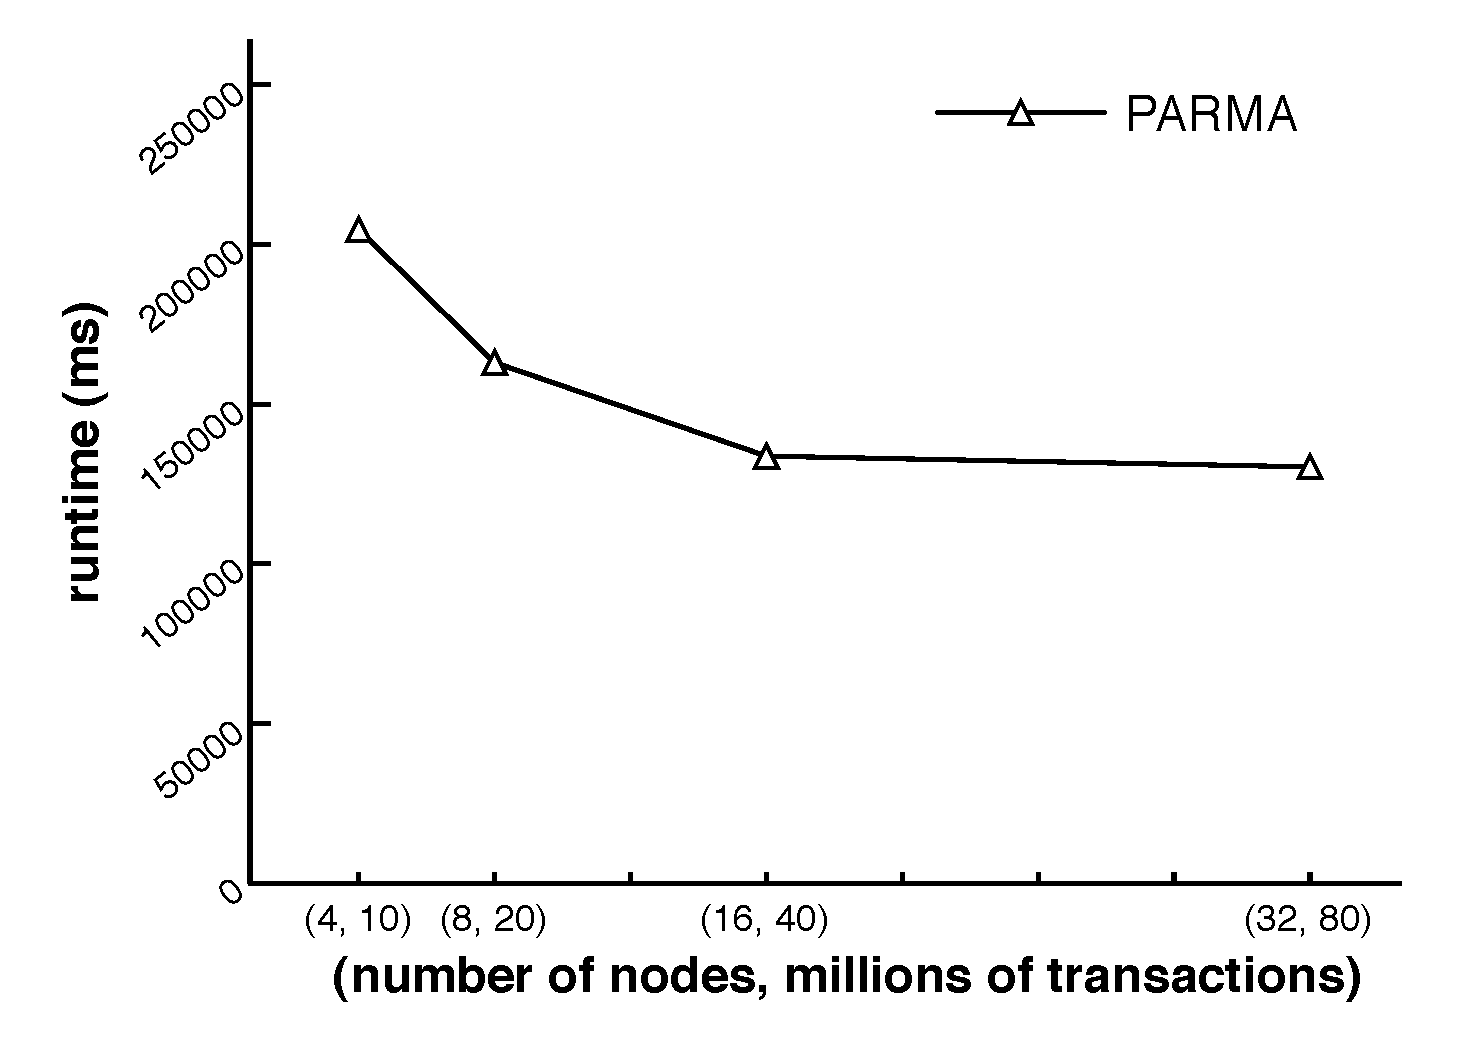
\includegraphics[width=\textwidth]{parma/scalability}
    \caption{Scalability as both data and cluster size are increased.}
    \label{fig:parmascalability}
  \end{subfigure}
  \caption{Speedup and scalability.}
\end{figure}

Also, as is clearly visible in the graph, the sub-ideal overall
speedup is due largely to the poor speedup of stage 2. Stage 2 is
bound almost entirely by the communication costs of transmitting the
local frequent itemsets from stage 1 to the reducers that will do the
aggregation. Because the amount of local frequent itemsets does not
change as more nodes are added, the communication for this stage does
not change. What does change is the number of itemsets each node must
aggregate. During the reduce phase, each node is assigned a set of
keys. All key/value pairs emitted from the map phase are sent to the
reducer assigned their respective key. The reducer is in charge of
aggregating the values and emitting one aggregate value per key assigned
to it. As more reducers are added to the cluster, each reducer will
have fewer keys assigned to it, and therefore must aggregate across
fewer values, resulting in faster aggregation. The small but existent positive
change in the line for stage 2 is a result of this slight speedup of the reduce
phase. 

Figure \ref{fig:parmascalability} depicts the scalability of PARMA as both
the size of the dataset (i.e. number of transactions) and the number of
nodes in the cluster are increased. The data and nodes are scaled
proportionally so that the ratio of data to nodes remains constant
across all experiments. This result shows that as nodes and data are
increased proportionally, the total runtime actually begins to decrease
for larger datasets. This is because as nodes are added to the cluster, the runtime of
the Stage 1 reducer (FIM) is decreased while the relative costs of
the Stage 1 mapper and Stage 2 remain the same. There is a leveling
off of the runtime between the 40M and 80M datasets, which can be
explained using Amdhal's law; because only portions of the algorithm
are parallelizable, there is a theoretical maximum speedup that is
possible. Still, the constant runtime as data is increased
demonstrates PARMA's potential scalability to real-world cluster and
dataset sizes. 

\begin{comment}
A very important aspect of PARMA that should be stressed again
here is that the size of the sample that will be mined does not depend
directly on size of the original database, but instead on the
confidence parameters $\varepsilon$ and $\delta$. From a practical
perspective, this means that assuming confidence parameters are
unchanged, larger and larger datasets can be mined with very little
increase in overall runtime (the added cost will only be the extra
time spent reading the larger dataset initially during
sampling). Because of this, clusters do not need to scale
with the data, and often a relatively modest cluster size will be
able to mine itemsets in a very reasonable time. 
\end{comment}

\subsection{Accuracy}
The output of PARMA is a collection of frequent itemsets which approximates the
collection one can obtain by mining the entire dataset. Although our analysis
shows that PARMA offers solid guarantees in terms of accuracy of the output, we
conducted an extensive evaluation to assess the actual performances of PARMA in
practice, especially in relation to what can be analytically proved.

We compared the results obtained by PARMA with the exact collection of
itemsets from the entire dataset, for different values of the parameters
$\varepsilon$, $\delta$, and $\theta$, and for different datasets. A first important
result is that in all the runs, the collection computed by PARMA was indeed an
absolute $\varepsilon$-close approximation to the real one, i.e., all the properties from
Definition~\ref{def:parmaeapproxfi} were satisfied. This fact suggests that the confidence in
the result obtained by PARMA is actually greater than the level $1-\delta$
suggested by the analysis. This can be explained by considering that we had to
use potentially loose theoretical bounds in the analysis to make it tractable. 

Given that all real frequent itemsets were included in the output, we then
focused on how many itemsets with real frequency in the interval
$[\theta-\varepsilon,\theta)$ were included in the output. It is important to
notice that these itemsets would be \emph{acceptable} false positives, as
Definition~\ref{def:parmaeapproxfi} does not forbid them to be present in the output.
We stress again that the output of PARMA never contained \emph{non-acceptable}
false positives, i.e. itemsets with real frequency less than the minimum
frequency threshold $\theta$. The number of acceptable false positives included in the
output of PARMA depends on the distribution of the real frequencies in the
interval $[\theta-\varepsilon,\theta)$, so it should not be judged in absolute
terms. In Table~\ref{tab:falsepositives} we report, for various values of
$\theta$, the number of real frequent itemsets (i.e., with real frequency at
least $\theta$, the number of acceptable false positives (AFP) contained in the output
of PARMA, and the number of itemsets with real frequency in the interval
$[\theta-\varepsilon,\theta)$, i.e., the maximum number of acceptable false
positives that may be contained in the output of PARMA (Max AFP). These numbers
refers to a run of PARMA on (samples of) the 10M dataset, with
$\varepsilon=0.05$ and $\delta=0.01$. It is evident that PARMA does a very good
job in filtering out even acceptable false positives, especially at lower
frequencies, when their number increases. This is thanks to the fact that  an
itemset is included in the output of PARMA if and only if it appears in the
majority of the collections obtained in the first stage. Itemsets with real frequencies
in $[\theta-\varepsilon,\theta)$ are not very likely to be contained in many of
these collections.

\begin{table}
  \centering
  \begin{tabular}{cccc}
    \hline
    $\theta$ & Real FI's & Output AFP's & Max AFP's \\
    \hline
    $0.06$ & 11016 & 11797 & 201636 \\
    $0.09$ & 2116& 4216& 10723 \\
    $0.12$ & 1367& 335& 1452\\
    $0.15$ & 1053& 299& 415\\
    \hline
  \end{tabular}
  \caption{Acceptable False Positives in the output of PARMA}
  \label{tab:falsepositives}
\end{table}

We conducted an evaluation of the accuracy of two other components of the
output of PARMA, namely the estimated frequencies for the itemsets in the output
and the width of the confidence bounds for these estimations. In
Figure~\ref{fig:parmaabsfreqerr} we show the distribution of the absolute error in
the estimation, i.e. $|\tilde{f}(X)-f_\Ds(X)|$ for all itemsets $X$ in the
output of PARMA, as $\theta$ varies. The lower end of the ``whisker'' indicates the minimum error,
the lower bound of the box corresponds to the first quartile, the segment across
the box to the median, and the upper bound of the box to the third quartile. The
top end of the whisker indicates the maximum error, and the central diamond
shows the mean. This figure (and also Figure~\ref{fig:parmaconfintwidth}) shows the values
for a run of PARMA on samples of the 10M dataset, with $\varepsilon=0.05$ and
$\delta=0.01$. We can see that even the maximum values are one order of
magnitude smaller than the threshold of $0.05$ guaranteed by the analysis, and
many of the errors are two or more orders of magnitude smaller. It is also
possible to appreciate that the distribution of the error would be heavily concentrated in a
small interval if the maximum error were not so high, effectively an outlier.
The fact that the average and the median of the error, together with the entire ``box'' move down as the
minimum frequency threshold decrease can be explained by the fact that at lower
frequencies more itemsets are considered, and this makes the distribution less
susceptible to outliers. Not only this is a sign of the high level of accuracy
achieved by PARMA, but also of its being consistently accurate on
a very large portion of the output.

\begin{figure}[htb]
 \centering
    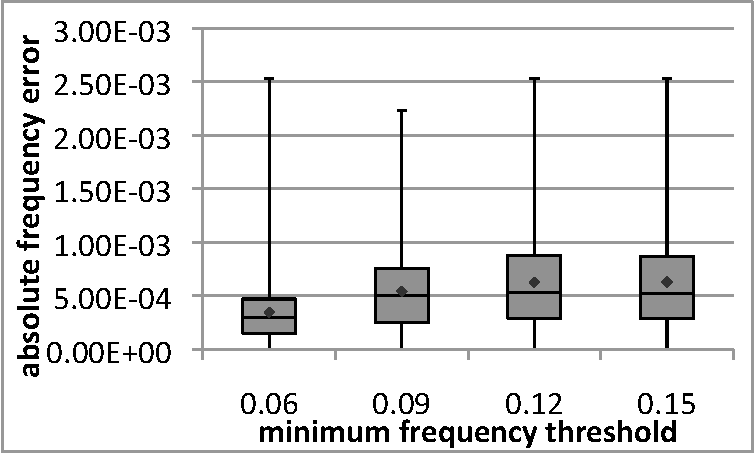
\includegraphics[width=0.3\textwidth]{parma/absfreqerr}
  \caption{Error in frequency estimations as frequency varies.}
  \label{fig:parmaabsfreqerr}
\end{figure}

\begin{figure}[htb]
 \centering
    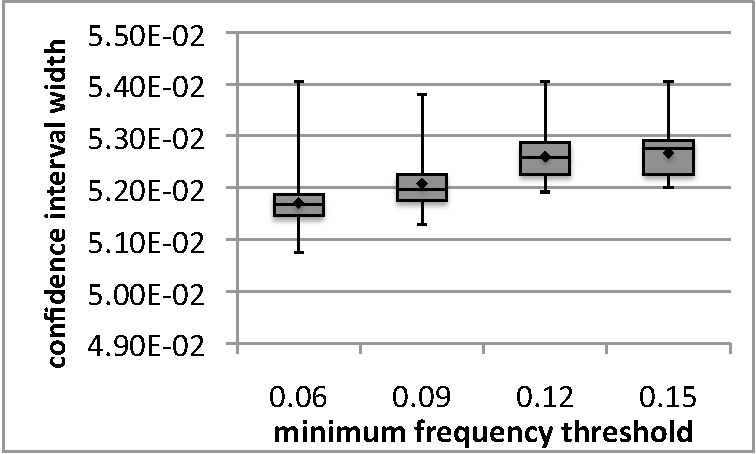
\includegraphics[width=0.3\textwidth]{parma/confintwidth}
  \caption{Width of the confidence intervals as frequency varies.}
  \label{fig:parmaconfintwidth}
\end{figure}

Finally, in Figure~\ref{fig:parmaconfintwidth} we show the distribution of the widths
of the confidence intervals $\mathcal{K}(A)$ for the frequency estimations
$\tilde{f}(A)$ of the itemsets $A$ in the output of PARMA. Given that
$\varepsilon=0.05$, the maximum allowed width was $2\varepsilon=0.1$. It is
evident from the figures that PARMA returns much narrower intervals, of size almost
$\varepsilon$. Moreover, the distribution of the width is very concentrated, as
shown by the small height of the boxes, suggesting that PARMA is extremely
consistent in giving very high quality confidence intervals for the estimations.
We state again that in all runs of PARMA in our tests, all the confidence
intervals contained the estimation and the real frequency, as requested by
Definition~\ref{def:parmaeapproxfi}. As seen in the case of the estimation
error, the distribution of the widths shifts down at lower thresholds $\theta$.
This is motivated by the higher number of itemsets in the output of PARMA at
those frequencies. Their presence makes the distribution more robust to
outliers. We can conclude that PARMA gives very narrow but
extremely accurate confidence intervals across the entirety of its output.

This analysis of the accuracy of various aspects of PARMA's output shows that
PARMA can be very useful in practice, and the confidence of the end user in
the collections of itemsets and estimations given in its output can be even higher
than what is guaranteed by the analysis.

